\documentclass[11pt,a4paper]{article}

\usepackage[utf8]{inputenc}
\usepackage[T1]{fontenc}
\usepackage{amsmath,amssymb,amsthm}
\usepackage{mathtools}
\usepackage{enumitem}
\usepackage{geometry}
\usepackage{aliascnt}
\usepackage{hyperref}
\usepackage{cleveref}
\usepackage{booktabs}
\usepackage{stmaryrd}
\usepackage{algorithm}
\usepackage{algpseudocode}

\geometry{margin=1in}

\newtheorem{definition}{Definition}[section]

\newaliascnt{condition}{definition}
\newtheorem{condition}[condition]{Condition}
\aliascntresetthe{condition}
\crefname{condition}{Condition}{Conditions}
\Crefname{condition}{Condition}{Conditions}

\newaliascnt{proposition}{definition}
\newtheorem{proposition}[proposition]{Proposition}
\aliascntresetthe{proposition}
\crefname{proposition}{Proposition}{Propositions}
\Crefname{proposition}{Proposition}{Propositions}

\newaliascnt{theorem}{definition}
\newtheorem{theorem}[theorem]{Theorem}
\aliascntresetthe{theorem}
\crefname{theorem}{Theorem}{Theorems}
\Crefname{theorem}{Theorem}{Theorems}

\newaliascnt{lemma}{definition}
\newtheorem{lemma}[lemma]{Lemma}
\aliascntresetthe{lemma}
\crefname{lemma}{Lemma}{Lemmas}
\Crefname{lemma}{Lemma}{Lemmas}

\newaliascnt{corollary}{definition}
\newtheorem{corollary}[corollary]{Corollary}
\aliascntresetthe{corollary}

\newaliascnt{remark}{definition}
\newtheorem{remark}[remark]{Remark}
\aliascntresetthe{remark}
\crefname{remark}{Remark}{Remarks}
\Crefname{remark}{Remark}{Remarks}

\DeclareMathOperator*{\argmax}{arg\,max}
\newcommand{\LL}{\mathcal{L}}
\newcommand{\XX}{\mathcal{X}}
\newcommand{\TT}{\mathcal{T}}
\newcommand{\Prior}{\textsc{Prior}}
\newcommand{\Likelihood}{\textsc{Likelihood}}
\newcommand{\Post}{\textsc{Post}}
\newcommand{\Expand}{\textsc{Expand}}
\newcommand{\Sever}{\textsc{Sever}}
\newcommand{\sem}[1]{\llbracket #1 \rrbracket}

\title{Bayesian Synthesis for Phylogenetic\\
Diversification Rate Models}
\author{PhyloBayesSynth}
\date{}

\begin{document}
\maketitle

\begin{abstract}
We present a Bayesian program synthesis framework for automatically
discovering phylogenetic diversification rate models from observed tree
data.  Models are represented as expressions in a probabilistic
domain-specific language (DSL) generated by a context-free grammar (CFG).
Synthesis is performed via Markov chain Monte Carlo (MCMC) over the space of DSL expressions.
\end{abstract}

\tableofcontents
\newpage

%% ====================================================================
\section{Method Overview}\label{sec:method}
%% ====================================================================

\subsection{Problem Statement}

Given a reconstructed phylogenetic tree consisting of a topology and
branch lengths for $n$ extant species, the goal is to automatically infer
both the \emph{form} (structure) and the \emph{parameters} of the
diversification rate model that best explains the observed tree under a
birth--death process. Here is a picture of the tree data we are modeling:
\begin{center}
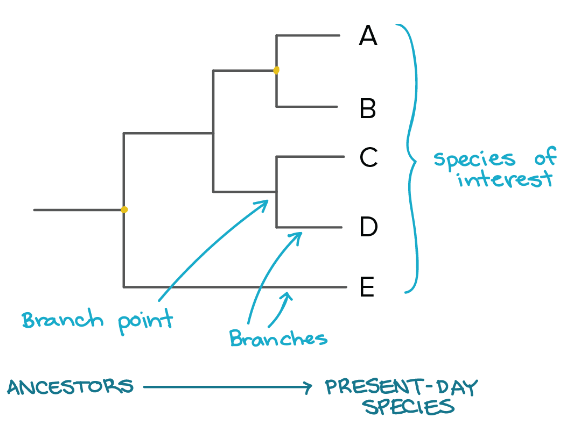
\includegraphics[width=0.5\textwidth]{tree.png}
\end{center}

\subsection{Domain-Specific Language}

We define a probabilistic DSL whose expressions are generated by the
following context-free grammar $G$:
\begin{align}
  N_1 &::= (\texttt{NoisyPhylo}\; N_2\; N_3) \notag\\
  N_2 &::= (\texttt{Noise}\; \Box) \notag\\
  N_3 &::= (\texttt{CRB}\; \Box)
       \mid (\texttt{CRBD}\; \Box\; \Box)
       \mid (\texttt{TDB}\; \Box\; \Box)
       \mid (\texttt{TDBD}\; \Box\; \Box\; \Box)
       \mid (\texttt{BAMM}\; \Box\; N_3\; N_3)
  \label{eq:grammar}
\end{align}
where $\Box$ denotes parameter holes filled by draws from continuous
prior distributions, and $N_1$ is the start symbol.  Each production of
$N_3$ corresponds to a diversification model class:
\begin{itemize}[nosep]
  \item \texttt{CRB}: constant-rate birth (Yule) process;
  \item \texttt{CRBD}: constant-rate birth--death;
  \item \texttt{TDB}: time-dependent birth (no extinction);
  \item \texttt{TDBD}: time-dependent birth--death;
  \item \texttt{BAMM}: introduces a Poisson change-point switching between a
    background ($\text{bg}$) and foreground ($\text{fg}$) sub-model,
    each of which is itself an $N_3$ expression (allowing recursive
    nesting).
\end{itemize}

\subsection{Prior Distribution}

Each production rule $r_{ik}$ for non-terminal $N_i$ is assigned a
selection probability $p_{ik} > 0$.  Parameters are drawn independently
from specified prior distributions (exponential, normal, beta, etc.).
The prior probability of an expression $E = (s, \theta)$ with structure
$s$ and parameters $\theta$ factorizes as
$\Prior\sem{E} = p_s \cdot \gamma_s(\theta)$, where $p_s$ is the
product of selection probabilities along the derivation and $\gamma_s$
is the product of parameter densities.

\subsection{Likelihood}

Each expression $E$ defines a generative process over phylogenetic
trees. \\
The likelihood $\Likelihood\sem{E}(O)$ of an observed tree $O$
is computed via:
\begin{itemize}[nosep]
  \item Closed-form expressions for pure-birth models.
  \item A unified ODE framework for models involving extinction and/or
    regime switching.
  \item A contamination-mixture noise model that interpolates between a
    structured model likelihood and a baseline noise likelihood.
\end{itemize}
\emph{Remark.} It is important to note that computing the likelihood for an isolated segment or a partial subtree is ill-posed. 
Because reconstructed phylogenetic trees are retrospectively conditioned on the sampling of extant species at the present day, the likelihood computation is only well-defined and meaningful when evaluated globally over the entire tree.
%% ====================================================================
\section{Convergence Theory}\label{sec:convergence}
%% ====================================================================

This section establishes that the MCMC synthesis algorithm
converges to the posterior distribution over DSL expressions.  We
follow the general framework of your PhD dissertation on Bayesian synthesis~\cite{saad2023}, adapting the
formalization to the phylogenetic setting.

\subsection{Probabilistic DSL Formalization}

\begin{definition}[Phylogenetic DSL]\label{def:dsl}
The phylogenetic domain-specific data modeling language $D$ is comprised
of:
\begin{itemize}[nosep]
  \item A countable structure space $S = \LL(G)$, the set of all
    s-expressions with parameter holes derivable from $G$;
  \item For each $s \in S$, a parameter space $\Theta_s$ equipped with
    sigma-algebra $\mathcal{F}_s$ and base measure $\lambda_s$ (products
    of Lebesgue measures on $\mathbb{R}$);
  \item An observation space $\XX$ consisting of all valid reconstructed
    phylogenetic trees with extant tips (\Cref{def:obs-space}).
\end{itemize}
\end{definition}

\begin{definition}[Observation space]\label{def:obs-space}
An observation $O \in \XX$ is a rooted phylogenetic tree with $n \geq 2$ extant tips.  Concretely, $O$ is
characterized by:
\begin{itemize}[nosep]
  \item A rooted labeled bifurcating topology $\mathfrak{t}$ with $n$
    leaves and $n - 1$ internal nodes
    $V_{\mathrm{int}} = \{v_1, \ldots, v_{n-1}\}$;
  \item Internal-node ages
    $(\tau_{v_1}, \ldots, \tau_{v_{n-1}}) \in \mathbb{R}_{>0}^{\,n-1}$
    satisfying $\tau_{\mathrm{pa}(v)} > \tau_v$ for every non-root
    $v \in V_{\mathrm{int}}$ (all leaves have age~$0$).
\end{itemize}
Each branch length is determined by
$\ell_e = \tau_{\mathrm{pa}(e)} - \tau_{\mathrm{child}(e)}$.  The tree
height is the root age $T = \max_v \tau_v$, the total branch length is
$S = \sum_e \ell_e$, and the branching times are the sorted internal-node
ages $\tau_1 > \tau_2 > \cdots > \tau_{n-1} > 0$.
\end{definition}

\begin{definition}[Likelihood semantics]\label{def:likelihood}
For each expression $E \in \LL$ and observation $O \in \XX$, the
likelihood $\Likelihood\sem{E}(O) \geq 0$ evaluates how well the
diversification model specified by $E$ explains the observed tree~$O$.
\end{definition}

\subsection{Conditions for Well-Defined Posterior}

Three conditions on the \Prior\ and \Likelihood\ semantics ensure that
the posterior $\Post\sem{E}(O)$ is a well-defined probability distribution for any fixed
observation~$O$.

% ---------- Condition: Normalized Prior ----------
\begin{condition}[Normalized Prior]\label{cond:prior}
The prior induces a probability distribution over $(\LL, \Sigma_\LL)$:
\begin{equation}
  \sum_{s \in S} \int_{\theta \in \Theta_s}
    \Prior\sem{(s,\theta)}\, \lambda_s(\mathrm{d}\theta) = 1.
  \label{eq:normalized-prior}
\end{equation}
\end{condition}

\begin{proposition}[Grammar Consistency]\label{prop:consistency}
The grammar $G$ in~\eqref{eq:grammar}, is consistent in the sense of Booth and
Thompson.
\end{proposition}

\begin{proof}
The non-terminals $N_1$ and $N_2$ are non-recursive (each has a single
production with no non-terminal children), so it suffices to verify
consistency of the $N_3$ sub-grammar.

\begin{alignat*}{3}
  &N_3 \to H_1\, H_0       &&\quad \tfrac{5}{20}\\
  &\phantom{N_3} \;\;\mid\; H_2\, H_0 &&\quad \tfrac{5}{20} \\
  &\phantom{N_3} \;\;\mid\; H_3\, H_0 &&\quad \tfrac{4}{20} \\
  &\phantom{N_3} \;\;\mid\; H_4\, H_0 &&\quad \tfrac{4}{20} \\
  &\phantom{N_3} \;\;\mid\; H_5\, N_3 &&\quad \tfrac{2}{20}
\end{alignat*}
\vspace{-1em}
\begin{alignat*}{2}
  H_0 &\to \Box
  &\qquad H_1 &\to \texttt{CRB} \\
  H_2 &\to H_6\, H_0
  &\qquad H_6 &\to \texttt{CRBD} \\
  H_3 &\to H_7\, H_0
  &\qquad H_7 &\to \texttt{TDB} \\
  H_4 &\to H_8\, H_0
  &\qquad H_8 &\to H_{10}\, H_0 \\
  H_5 &\to H_9\, N_3
  &\qquad H_9 &\to H_{11}\, H_0 \\
  H_{10} &\to H_{12}\, H_0
  &\qquad H_{11} &\to \texttt{BAMM} \\
  H_{12} &\to \texttt{TDBD}
\end{alignat*}

Following Gecse and Kov{\'a}cs, define
$m_{ij} = \sum_{k=1}^{r_i} p_{ik}\, n_{ikj}$,
The expectation matrix $M = [m_{ij}]$ is:
\begin{equation}\label{eq:expectation-matrix}
\setlength{\arraycolsep}{2.5pt}
\footnotesize
M = \left(\begin{array}{cccccccccccccc}
\frac{2}{20} & \frac{18}{20} & \frac{5}{20} & \frac{5}{20} & \frac{4}{20} & \frac{4}{20} & \frac{2}{20} & 0 & 0 & 0 & 0 & 0 & 0 & 0 \\[2pt]
0&0&0&0&0&0&0&0&0&0&0&0&0&0\\
0&0&0&0&0&0&0&0&0&0&0&0&0&0\\
0&1&0&0&0&0&0&1&0&0&0&0&0&0\\
0&1&0&0&0&0&0&0&1&0&0&0&0&0\\
0&1&0&0&0&0&0&0&0&1&0&0&0&0\\
1&0&0&0&0&0&0&0&0&0&1&0&0&0\\
0&0&0&0&0&0&0&0&0&0&0&0&0&0\\
0&0&0&0&0&0&0&0&0&0&0&0&0&0\\
0&1&0&0&0&0&0&0&0&0&0&1&0&0\\
0&1&0&0&0&0&0&0&0&0&0&0&1&0\\
0&1&0&0&0&0&0&0&0&0&0&0&0&1\\
0&0&0&0&0&0&0&0&0&0&0&0&0&0\\
0&0&0&0&0&0&0&0&0&0&0&0&0&0
\end{array}\right).
\end{equation}

The nonzero eigenvalues of $M$ are 0.3702... and -0.2702... which lie in the interval [-1,1].
By Theorem~3.35 of~\cite{saad2023}, $G$ is
consistent.
\end{proof}
Since $G$ is consistent and the parameter distributions $\mu_{ik}$ are
probability measures, \Cref{cond:prior} holds by the factorization
$\Prior\sem{(s,\theta)} = p_s \cdot \gamma_s(\theta)$ and the fact that
$\sum_{s \in S} p_s = 1$ and
$\int_{\Theta_s} \gamma_s(\theta)\,\lambda_s(\mathrm{d}\theta) = 1$.


% ---------- Condition: Positive Likelihood ----------
\begin{condition}[Positive Likelihood]\label{cond:pos-lik}
For each observation $O \in \XX$, there exists a set $A \subset \LL$ of
positive prior measure such that $\Likelihood\sem{E}(O) > 0$ for all
$E \in A$.
\end{condition}

\begin{proof}
Since $S > 0$ for any valid tree, the \texttt{CRB} likelihood
$\Gamma(n)\,\lambda^{n-1} e^{-\lambda S}$ is strictly positive for all
$\lambda > 0$.  And the set of \texttt{CRB} expressions has positive prior
measure.
\end{proof}
% ---------- Condition: Bounded Likelihood ----------
\begin{condition}[Bounded Likelihood]\label{cond:bdd-lik}
For each observation $O \in \XX$, the likelihood is essentially bounded:
there exists a finite constant $c^{\max}_{O} > 0$ such that
$\{E \in \LL \mid \Likelihood\sem{E}(O) > c^{\max}_{O}\}$ has
prior measure zero.
\end{condition}

\begin{proof}
Let $E = (\texttt{NoisyPhylo}\;(\texttt{Noise}\;\sigma)\;M)$ with
$\pi = \sigma/(1+\sigma) \in [0,1)$.  The final likelihood satisfies
\begin{equation}\label{eq:lik-split}
  \Likelihood\sem{E}(O)
  = (1-\pi)\,\LL_{\mathrm{model}}(M, O)
  + \pi\,\LL_{\mathrm{noise}}(O)
  \leq \LL_{\mathrm{model}}(M, O) + \LL_{\mathrm{noise}}(O).
\end{equation}
The noise baseline is
$\LL_{\mathrm{noise}}(O) = \beta\,[\Gamma(n)]^2 / (S+\beta)^n$, where
$\beta = 1/\text{scale}_\lambda$ is a fixed hyperparameter of the
prior, and $n$, $S$ are determined by the fixed tree~$O$.  For any
given~$O$, this is a finite positive constant independent of the
expression~$E$.\\
It remains to show that $\LL_{\mathrm{model}}(M, O)$ is bounded
independently of the expression~$M$.  We treat each model class in
turn.

\emph{Pure-birth models} (\texttt{CRB}, \texttt{TDB}).  Both have
closed-form likelihoods of the form
$\LL = \Gamma(n) \prod_{k=1}^{n-1} \lambda(\tau_k)
\cdot e^{-\sum_i \Lambda_i}$,
where $\Lambda_i = \int_{\tau_c^{(i)}}^{\tau_p^{(i)}} \lambda(\tau)\,
\mathrm{d}\tau > 0$.  For \texttt{CRB} ($\lambda(\tau) \equiv \lambda$),
this gives $\Gamma(n)\,\lambda^{n-1} e^{-\lambda S}$, maximized at
$\lambda^* = (n-1)/S$ with finite maximum
$\Gamma(n)\,((n-1)/(eS))^{n-1}$, independent of~$\lambda$.
For \texttt{TDB} ($\lambda(\tau) = \lambda_0 e^{z(T-\tau)}$), the
likelihood is a continuous function that vanishes at
every boundary of the parameter space, so it attains a finite
supremum.

\emph{Birth--death models} (\texttt{CRBD}, \texttt{TDBD},
\texttt{BAMM}).  The likelihood takes the ODE-based form
$\Gamma(n)\,D_{\mathrm{root}} / (1 - E(T))^2$.  The ODE solutions
$D_{\mathrm{root}}$ and $E(T)$ are continuous functions of the rate
parameters.  At degenerate boundaries ($\lambda \to 0$,
$\mu \to \infty$, or $E(T) \to 1$) the likelihood vanishes
($\log \LL = -\infty$); at the opposite extreme ($\mu = 0$) it reduces
to a pure-birth model bounded as above. So they attain finite suprema.
\end{proof}

\begin{proposition}[Well-Defined Posterior]\label{prop:posterior}
If \Cref{cond:prior,cond:pos-lik,cond:bdd-lik} hold and the
likelihood is measurable, then for any fixed observation $O \in \XX$,
the posterior $\Post\sem{E}(O) \propto \Likelihood\sem{E}(O) \cdot
\Prior\sem{E}$ is a well-defined probability distribution over
$(\LL, \Sigma_\LL)$.
\end{proposition}
\begin{proof}
The proof is identical to Propositions~3.11--3.12
of~\cite{saad2023}: \Cref{cond:pos-lik} gives $c_O > 0$ and
\Cref{cond:bdd-lik} with \Cref{cond:prior} gives $c_O < \infty$.
\end{proof}
\subsection{Transition Operator}

Our transition operator is an instance of Algorithm~3.3
of~\cite{saad2023} applied to the phylogenetic grammar~$G$: uniformly
select a node~$a$ in the parse tree, sever the subexpression at~$a$ to
obtain a non-terminal~$N_i$, re-expand from~$N_i$ via \Expand, and
accept the proposal with Metropolis--Hastings probability
\begin{equation}
  \alpha(E, E') = \min\!\left\{
    1,\;
    \frac{|A_E|}{|A_{E'}|}
    \cdot
    \frac{\Likelihood\sem{E'}(O)}{\Likelihood\sem{E}(O)}
  \right\},
  \label{eq:mh-accept}
\end{equation}
where $|A_E|$ is the number of nodes in the parse tree of~$E$.

Since our grammar is context-free, the three conditions required by the
MCMC convergence theory are all satisfied by the proofs of
Lemmas~3.50--3.52 of~\cite{saad2023}, which apply to any
context-free probabilistic DSL without modification.

\subsection{Main Convergence Results}

\begin{theorem}[MCMC Convergence in Total Variation]\label{thm:mcmc-tv}
Let $O \in \XX$ be an observation and $E_0 \in \LL$ satisfy
$\Likelihood\sem{E_0}(O) > 0$.  Let $(E_1, \ldots, E_n)$ be the
output of the MCMC algorithm (Algorithm~3.1 of~\cite{saad2023}) using
the transition operator described above.  Then
\begin{equation}
  \sup_{\mathcal{E} \subset \LL}
  \left|
    \sum_{E \in \mathcal{E}}
    \bigl[\mathrm{ApproxPost}^{(n)}_{E_0}\sem{E}(O)
    - \Post\sem{E}(O)\bigr]
  \right|
  \xrightarrow{n \to \infty} 0.
\end{equation}
\end{theorem}

\begin{proof}
Lemmas~3.50--3.52 of~\cite{saad2023} verify posterior invariance,
irreducibility, and aperiodicity for the transition operator.  The
result follows from Theorem~3.19 of~\cite{saad2023}.
\end{proof}

\begin{theorem}[Strong Law of Large Numbers for MCMC]\label{thm:mcmc-lln}
Under the hypotheses of \Cref{thm:mcmc-tv}, for any function
$\varphi : \LL \to \mathbb{R}$ satisfying
$\sum_{E \in \LL} |\varphi(E)| \cdot \Post\sem{E}(O) < \infty$,
\begin{equation}
  \frac{1}{n} \sum_{i=1}^{n} \varphi(E_i)
  \xrightarrow{n \to \infty}
  \sum_{E \in \LL} \varphi(E) \cdot \Post\sem{E}(O)
  =: \mathbb{E}_{\Post}[\varphi(E)]
  \qquad \text{almost surely}.
\end{equation}
\end{theorem}

\begin{proof}
Follows from Theorem~3.20 of~\cite{saad2023}.
\end{proof}

%% ====================================================================
\section{Evaluation \& Questions}\label{sec:evaluation}
%% ====================================================================

To verify the correctness of the algorithm, we generate a phylogenetic tree from a known model structure and run the MCMC algorithm to attempt to recover this true structure.\\
The original structure is CRBD(0.09, 0.02), noise=0, log L = -12.0640.\\
But the best expression found is (BAMM 0.0311 (TDBD 0.1462 -0.4111 0.0783) (CRBD 0.1164 0.0073)), noise=0.0207, log L = -8.9632\\
This raises several questions:

\begin{itemize}
\item \textbf{Maximum Likelihood?} Why does the global maximum-likelihood expression differs from the true generative structure? Does this discrepancy indicate a bug in our implementation, or a flaw in the convergence proofs established in Section~\ref{sec:convergence}? Or is this behavior entirely expected?

\item \textbf{Overfitting?} Do complex structures naturally achieve higher likelihoods simply by having more free parameters to fit stochastic noise?
Our attempt runs show that data generated by \texttt{CRBD} correctly yields \texttt{CRBD} as the most frequently visited structure on the chain, but with less log-likelihood than BAMM. Does this imply we should adopt the highest posterior frequency structure as our primary result, while maintaining a separate maximum-likelihood expression for each expression class?
\end{itemize}
%% ====================================================================
\section*{Acknowledgments}
%% ====================================================================
The framework closely follows methods introduced in ~\cite{saad2023}.\\
We are very impressed by your dissertation on Bayesian synthesis.

%% ====================================================================
\begin{thebibliography}{99}

\bibitem{saad2023}
Feras Ahmad Khaled Saad,
\emph{Scalable Structure Learning, Inference, and Analysis with Probabilistic Programs},
Ph.D.\ thesis, MIT, 2022.
Chapter~3: Synthesizing Probabilistic Programs in Domain-Specific
Modeling Languages.

\end{thebibliography}

\end{document}
